%
% Modelo LaTeX baseado no modelo A5L
% Adaptação para LaTeX por Bruno Ferreira

% Nota: usar /newpage com 1 coluna
%       usar /clearpage com 2 colunas
%       o /newpage com duas colunas escreve na próxima 
\documentclass[a5paper,twocolumn, 11pt]{article}
\usepackage[landscape]{geometry}

%Sample text
\usepackage{lipsum}

%escrever acentos e coisas do género sem que o latex se desoriente
\usepackage[utf8]{inputenc}

%hifenização e titulos em português
\usepackage[portuges]{babel}

%para ter a informação de quantas páginas tem o documento
\usepackage{lastpage}

%importar cores predefinidas
\usepackage[usenames,dvipsnames]{xcolor}
\definecolor{DarkGray}{gray}{0.40}

%usar multirow e multicolumn
\usepackage{multirow}

%para ter imagens, depois define a directoria de imagens
\usepackage{graphicx}
\graphicspath{{./imagens/}}

%definir o cabeçalho e rodapé
\usepackage{fancyhdr}
\pagestyle{fancy}
\fancyhead[L]{
    \small{
        \textcolor{DarkGray}{
            \textbf{Uminho 2012 - LI3 --- Transitários LEI}
        }
    }
}
\fancyhead[R]{
    \small{
        \textcolor{DarkGray}{
            \textbf{Pág. \thepage\ /\pageref{LastPage}}
        }
    }
}
\fancyfoot[C]{}

%definir regras de hifenização
\hyphenation{
chaining
Hash
}

%definir comando \hyph{}, necessário para n\hyph{}dimensionais
\def\hyph{-\penalty0\hskip0pt\relax}

\begin{document}

\onecolumn
\thispagestyle{empty}
\begin{tabular}{ll}
    \multirow{7}{*}{ 
\includegraphics[height=90pt]{logo.jpeg} }
    &\\
    & \textcolor{DarkGray}{\Large{\textbf{Escola de Engenharia}}} \\
    &\\
    & \large{Departamento de Informática}\\
    &\\
    &\\
    & \large{Licenciatura em Engenharia Informática}\\
\end{tabular}
\begin{center}
    \Large{\textbf{Projecto de Laboratórios de Informática III}}\\
    \vspace{20pt}
    \Large{\textbf{``Transistários LEI --- Transporte de Carga''}}\\
    \vspace{15pt}
    \begin{tabular}{r@{, }l}
        Bruno Ferreira&A61055\\
        Daniel Carvalho&A61008\\
        Mariana Madeiros&A61041\\
    \end{tabular}
    
    \vspace{5pt}
    \emph{Grupo 42}\\\vspace{15pt}
    \large{\textbf{Braga, Março de 2012}}
\end{center}

\newpage
\twocolumn
\tableofcontents
\newpage
\listoffigures

\newpage
\section{Resumo}
Neste relatório encontram-se explicitadas de forma detalhada as escolhas do \mbox{grupo 42} no que ao projecto da unidade curricular de \mbox{Laboratórios de Informática III} diz respeito. Serão revistas as escolhas em relação às estruturas de dados usadas, a forma como se interligam, a complexidade algorítmica sobre essas mesmas estruturas e outras opções relativas à abordagem do problema que nos é exposto no projecto.

Relativamente às estruturas de dados será feita uma abordagem sobre módulos genéricos e a forma como estes foram tidos em conta como uma possível solução para o problema assim como a implementação na mesma solução.

Para além do já supracitado este relatório serve de referência para o uso da interface do programa pelo utilizador, sendo explicado com pormenor o uso e o funcionamento desta.

\clearpage
\section{Introdução}
Uma empresa de transportes de nome Transitários LEI procura uma solução informática que permita registar informação relativa aos seus serviços bem como auxiliar a empresa na execução dos mesmos.

É da pretensão da administração da empresa possuir uma base de dados de localidades para e de onde é possível fazer transporte, de clientes, de meios de transportes disponíveis e serviços prestados.

Atendendo às várias restrições que a empresa comporta nos seus serviços como a não existência de dupla direcção de ligações entre duas localidades, prevê-se que seja necessário que o programa execute várias tarefas, fazendo-se notar as seguintes:
\begin{itemize}
    \item{Inserção e remoção de localidades;}
    \item{Inserção e remoção de ligações entre localidades;}
    \item{Alteração das propriedades de localidades e das ligações entre estas;}
    \item{Inserção, remoção e edição tanto de clientes como dos meios de transporte possuídos pela empresa}
    \item{Registo dos serviços prestados}
\end{itemize}
Tendo estas informações como base irá de seguida ser mostrado o processo de análise e
solução do problema apresentado implementado na linguagem imperativa C.

\clearpage
\section{Conteúdo}
\subsection[Estruturas de dados]{Estruturas de dados -- Abordagem geral ao problema}
\label{abordagem geral}
Tendo em conta o problema apresentado pela empresa Transitários LEI chegou-se a uma possível solução que prova ser eficiente na execução das tarefas que são necessárias satisfazer. De forma sucinta presentemente, e mais à frente neste relatório de forma mais detalhada, passa-se então à explicação das escolhas das estruturas de dados para a implementação de uma solução que satisfaça os requisitos da empresa. Dividindo o problema em duas partes, no âmbito do tipo de dados a tratar temos de um lado localidades e do outro clientes e camiões.

No caso das localidades, optou-se por usar uma estrutura que fosse eficiente o suficiente para oferecer ao utilizador uma robustez suficiente para lidar com uma grande gama em termos de quantidade de localidades e ao mesmo tempo que oferece-se rapidez na procura. A solução idealizada e que foi de facto implementada foi uma Tabela de Dispersão (‘Hash Table’) com encadeamento (‘Chaining’), ou seja, em cada uma das posições da tabela é utilizado um apontador para uma lista ligada de localizações de forma a evitar colisões na tabela. Também é de referir que a cada localidade estão associadas duas listas ligadas que indicam as localidades a que uma determinada localidade está associada por ligação. Esta solução traz à solução uma rapidez considerável assim como uma inserção igualmente rápida comparativamente a outras estruturas de dados.

Relativamente aos camiões e clientes, a solução encontrada foi utilizar uma árvore binária AVL, ou seja uma árvore binária de procura balanceada por altura, mas com a particularidade de ter n\hyph{}dimensões, ou seja, torna-se possível balancear uma única árvore de tendo em conta diferentes critérios sem a necessidade de recorrer à criação de uma outra árvore binária.

Tendo em conta a necessidade de procurar intensivamente tanto clientes como camiões, este tipo de estrutura beneficia de forma acentuada o acesso aos dados e apesar de incorrer em falta no que à inserção e balanceamento diz respeito, é necessário notar que uma pesquisa de clientes é uma operação utilizada de forma bem mais rotineira que uma inserção, logo este pequeno obstáculo à eficiência, faz-se provar não tão grave quando comparado com a eficiência que nos é dada relativamente à pesquisa.


\clearpage
\subsection[Localidades]{Localidades -- Tabela de Hash com chaining, Grafos e Listas Ligadas}
Uma tabela de dispersão permite operações sobre os elementos desta bastante rápidos e eficientes pois é possível encontrar um elemento através de uma `hashkey', ou chave de dispersão, que associa imediatamente o elemento a uma posição do array, tanto para pesquisas como inserções ou remoções. Essa associação muitas vezes resulta em colisões, ou seja, a função que gera as chaves de dispersão pode gerar a mesma chave para dois elementos diferentes o que impediria a inserção, por exemplo, de outro elemento com a mesma chave numa determinada posição do array já ocupada. Como forma de resolver este problema optou-se pela utilização de encadeamento sobre a tabela de dispersão, ou seja, para cada posição do array é possível introduzir todos os elementos que fiquem associados a ele através da sua chave de dispersão usando listas ligadas, evitando assim colisões. Para este caso em concreto um rápido acesso às localidades traduz-me numa vantagem enorme na implementação de
algoritmos sobre estas.

Usando o conceito de grafo, é possível introduzir uma localidade na tabela de dispersão, e vendo essa localidade como um vértice de um grafo, é possível adicionar a cada localidade uma lista de adjacências, ou seja, para este caso propriamente dito, duas listas que indicam quais as localidades que se ligam a uma determinada localidade assim como as localidades que estão ligadas a essa mesma localidade.

Como é necessário que o programa mostre robustez a lidar com um grande número de localidades, a tabela de dispersão está preparada para fazes escalonamento sempre que se torne evidente que está a ficar com um factor de carga elevado, o que também prejudica a dispersão na tabela.

A implementação foi baseada em módulos genéricos de Tabelas de dispersão e listas ligadas capazes de lidar com a situação já descrita. Em termos de complexidade algorítmica, o acesso aos dados é de $1+n$ em que $n$ é o número de elementos da lista nessa posição da tabela. Mas tendo em conta que assim que o factor de carga da tabela de hashing seja superior a metade do tamanho da tabela, esta é escalada para o seu dobro, a dispersão é muito mais eficiente e as listas serão em seu tamanho diminutas. Assim, a utilização de listas não afectará de forma notável o desempenho da aplicação. Para as listas ligadas a complexidade algorítmica é $O(n)$.

Seguindo-se neste relatório encontram-se duas figuras ilustrativas da forma como as localidades usam as estruturas de dados acima referidos, de uma forma mais genérica.

IMAGEM

IMAGEM

\clearpage
\subsection[Clientes e Camiões]{Clientes e Camiões -- Árvores AVL n\hyph{}dimensionais}
As árvores Adelson-Velskii Landis n\hyph{}dimensionais surgiram da necessidade de ordenar o mesmo conjunto de informação de várias formas diferentes, isto sem ocupar demasiado espaço em memória.

As árvores AVL são árvores binárias balanceadas de modo a terem sempre complexidade logarítmica de base 2 ($\log_2 n$). Cada nodo de uma árvore AVL é constituído por:
\begin{itemize}
\item{Apontador para o nodo à esquerda;}
\item{Apontador para o nodo à direita;}
\item{Indicador da altura do nodo;}
\item{Apontador para os dados.}
\end{itemize}
Usar árvores binárias AVL, pelos motivos enunciados na \emph{Abordagem geral ao problema} (Secção \ref{abordagem geral}), é a melhor forma de organizar a informação relativa a clientes e camiões. Mas para termos a informação optimizada para pesquisa precisávamos de ter tantas árvores binárias quantos os campos pelos quais queríamos ordenar a informação. Como isso seria um desperdício de memória, procurou-se uma alternativa que solucionasse o nosso problema sem ocupar muitos recursos. Assim surgiram as AVL n\hyph{}dimensionais.
\begin{figure}[hbt]
    \caption[Nodo AVL n\hyph{}dimensional]{Nodo AVL n\hyph{}dimensional.}
    \label{nodo avl ndimensional}
    \centering
        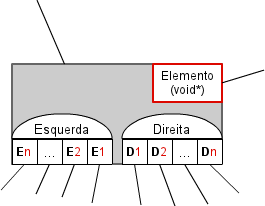
\includegraphics[width=180pt]{nodo_ndavl.png}
\end{figure}
\begin{figure}[hbt]
    \caption[Representação lógica AVL bi\hyph{}dimensional]{Representação lógica de uma AVL bi\hyph{}dimensional}
    \label{duas avl comuns}
    \centering
        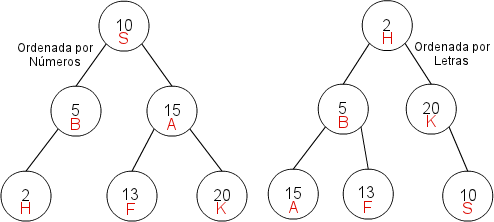
\includegraphics[width=170pt]{duas_avl_comuns.png}
\end{figure}

As AVL n\hyph{}dimensionais não são mais que várias árvores AVL que partilham o espaço em memória e estão organizadas logicamente de maneiras distintas, fazendo para esse efeito, uso de um conjunto de apontadores para nodos à esquerda e à direita, em vez de apenas um para cada direcção. Esse conjunto (array) de apontadores permite fazer a distinção entre as várias dimensões, assim como ter a possibilidade de ajustar o código para comportar mais dimensões. Cada posição do array define uma ``dimensão'' da árvore, ou seja, uma maneira diferente de organizar a informação tendo em conta critérios de procura distintos.
As árvores binárias AVL de n\hyph{}dimensões são assim compostas por:
\begin{itemize}
\item{Apontadores para os nodo à esquerda (array);}
\item{Apontadores para os nodo à direita (array);}
\item{Indicadores da altura do nodo (array);}
\item{Apontador para os dados.}
\end{itemize}
É necessário ter vários indicadores de altura para o mesmo nodo, pois a altura do nodo depende de uma organização específica e diferente para cada dimensão da árvore. Pode-se ter uma noção mias clara da organização de um nodo AVL n\hyph{}dimensional pela observação da figura~\ref{nodo avl ndimensional}.

Com o auxílio das figuras~\ref{nodo avl ndimensional} e~\ref{duas avl comuns} consegue-se perceber que uma AVL com n\hyph{}dimensões não é mais que $n$ árvores binárias que partilham o espaço de memória.

\clearpage
\subsection{Interface}
A interface da aplicação foi desenvolvida de forma a ser independente do resto da solução. O módulo de interface tem apenas duas funções: mostrar um menu e fazer uso de funções externas para responder ao input do utilizador.
\begin{figure}[hbt]
    \caption[Menu Principal]{Menu Principal}
    \label{menu principal}
    \centering
        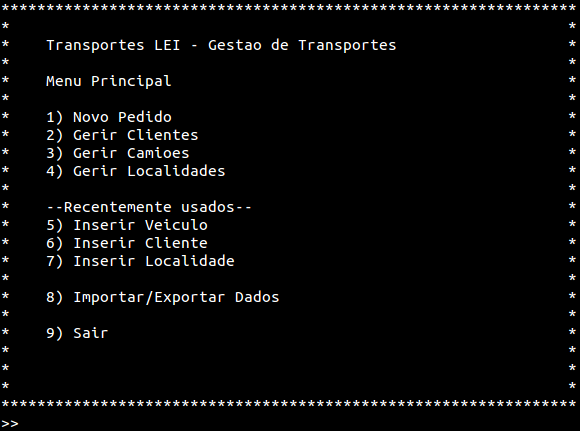
\includegraphics[width=200pt]{menu_principal.png}
\end{figure}
\begin{figure}[hbt]
    \caption[Menu Gestão Clientes]{Menu de Gestão de Clientes}
    \label{menu gerir clientes}
    \centering
        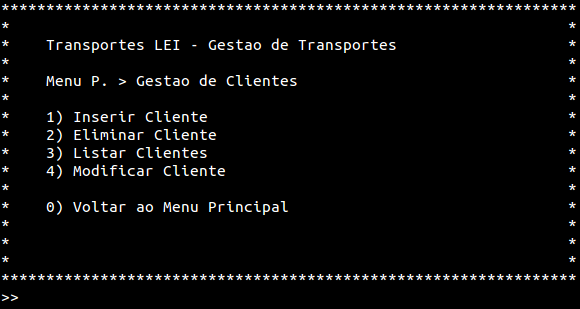
\includegraphics[width=200pt]{menu_gestao_de_clientes.png}
\end{figure}

A interface foi desenhada para ser simples e poderosa, isto é, ao mesmo tempo que permite ao utilizador comum a utilização do programa, deixa que o utilizador avançado utilize atalhos e combinações de números para navegar rapidamente pelos menus e sub-menus.
Existem duas implementações dignas de destaque no módulo de interface:


A primeira é a possibilidade de introduzir uma sequência de números para navegar pelos menus de forma mais rápida, isto é, imagine-se a seguinte situação: o utilizador, para realizar determinada acção, tem de escolher a segunda opção do menu, seguida da primeira opção de um sub-menu e depois escolher ainda a terceira opção de um sub-menu deste ultimo. Em vez disto, o utilizador pode introduzir (neste caso)~213 no menu principal e a aplicação executará imediatamente a acção determinada.

A segunda implementação consiste na apresentação de três atalhos no menu principal que correspondem precisamente às três últimas funções solicitadas pelo utilizador. Assim aumenta-se a produtividade de um utilizador que realize tarefas repetitivas.
Nas figuras~\ref{menu principal} e~\ref{menu principal com atalho diferente} pode-se observar uma alteração nos atalhos apresentados.
\begin{figure}[hbt]
    \caption[Menu Principal (atalho)]{Menu com atalho diferente}
    \label{menu principal com atalho diferente}
    \centering
        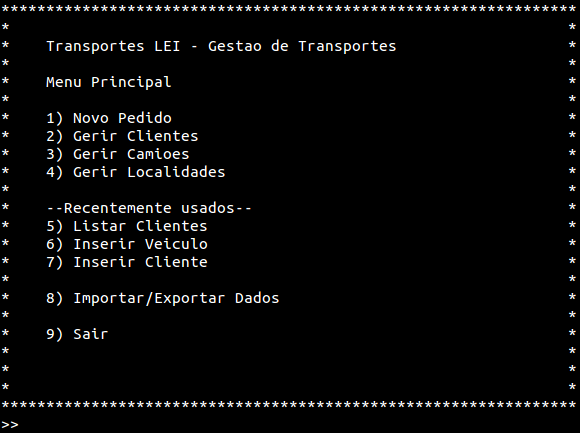
\includegraphics[width=200pt]{menu_com_atalho_diferente.png}
\end{figure}



\clearpage
\section{Conclusão}
Este relatório serve de referência para as soluções e implementações que, tendo em conta todas as indicações dadas pelo enunciado do projecto, foram tidas em conta pelo grupo. De forma sucinta a escolha passou por Tabela de Hash com chaining utilizando o conceito de grafo e listas ligadas para tratamento de localidades e árvores AVL n\hyph{}dimensionais para o tratamento de clientes e camiões.

Durante a fase de trabalhos do grupo recorreu-se ao git devido à sua capacidade de controlo de versões.

De saudar também o empenho dos elementos do grupo que trabalharam afincadamente na realização desta etapa do projecto.

\clearpage
\onecolumn
\section{Fotos}
\begin{center}
    \begin{tabular}{ccc}
        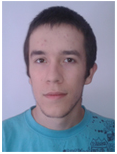
\includegraphics[width=90pt]{bruno.png}&
        
\includegraphics[width=90pt]{daniel.png}&
        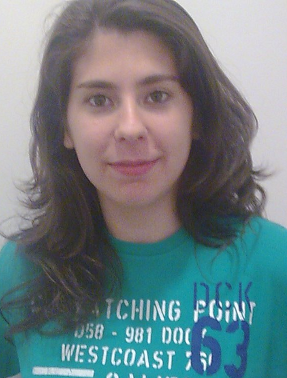
\includegraphics[width=90pt]{mariana.png}\\
        
        \small{\textbf{Bruno Ferreira}}&
        \small{\textbf{Daniel Carvalho}}&
        \small{\textbf{Mariana Medeiros}}\\
        \small{\textbf{A61055}}&
        \small{\textbf{A61008}}&
        \small{\textbf{A61041}}\\
    \end{tabular}
\end{center}
\end{document}